% ######################################################################################################################
%         Visualization
% ######################################################################################################################

\chapter{Visualization}
\label{ch:Visualization}

\paperbox{
    This chapter is based on the peer-reviewed publication:
}{\paperpppp}{
    \textbf{Contributions:} Lucas Czech... Alexandros Stamatakis...
}

% ######################################################################################################################
%         Motivation
% ######################################################################################################################

\section{Motivation}
\label{ch:Visualization:sec:Motivation}

A first step in analyzing phylogenetic placement data is often to visualize them.
For small samples, it is possible to mark individual placement locations on the \ac{RT},
as offered for example by \toolname{iTOL} \cite{Letunic2016},
or even to create a tree where the most probable placement per \ac{QS} is attached as a new branch,
as implemented in the \toolname{guppy} tool from the \toolname{pplacer} suite \cite{Matsen2010},
\toolname{RAxML-EPA} \cite{Berger2011,Stamatakis2014}, and our tool \toolname{gappa}.
For larger samples, one can alternatively display the per-edge placement mass,
either by adjusting the line widths of the edges according to their mass, or by using a color scale,
as offered in \toolname{ggtree} \cite{Yu2017}, \toolname{guppy}, and \toolname{gappa}.
Using per-edge colors corresponds to binning all placement of an edge into one bin.
%it is thinkable to use multiple bins instead, too, resulting in edges split into segments with different colors.
For large datasets, the per-edge masses can vary by several orders of magnitude.
In these cases, it is often preferable to use a logarithmic scaling, as shown in \cite{Mahe2017}.
%In addition to visualizing each sample separately, the average mass distribution gives an overview of a set of samples.

These simple visualizations directly depict the placement masses on the tree.
When visualizing the accumulated masses of multiple samples at once,
it is important to chose the appropriate normalization strategy for the task at hand.
For example, if samples represent different locations, one might prefer to use normalized masses,
as comparing relative abundances is common for this type of data.
On the other hand, if samples from the same location are combined
(e.g., from different points in time, or different size fractions),
it might be preferable to use absolute abundances instead,
so that the total number of sequences per sample can be visualized.

The visualizations provide an overview of the species abundances over the tree.
They can be regarded as a more detailed version of classic abundance pie charts.
When placing OTUs, or ignoring sequence abundances, the resulting visualizations depict species diversity.
% Those two figures can even be combined into one by adding brackets with abundances
% around the clades of the tree when drawing it.
% When drawing the tree, abundances can also be annotated around its clades,
% effectively combining those two figures into one.
Moreover, these visualizations can be used to assess the quality of the \ac{RT}.
% No ``zone'' here? Micah will be disappointed...
% The inner edges of the \ac{RT} form a zone of older evolutionary relationships.
% Placements into that zone may indicate that appropriate reference sequences
For example, placements into inner branches of the \ac{RT} may indicate that appropriate reference sequences
(i) have not been included or (ii) are simply not yet available.
%This complements the sequence filtering that relies on so-called backbone trees
% as described in \nameref{sec:Preprocessing::sub:MultilevelPlacement}.
%that we recently introduced \cite{Czech2018}.

Here, we introduce visualization methods that highlight
(i) regions of the tree with a high variance in their placement distribution (called \emph{Edge Dispersion}),
and (ii) regions with a high correlation to meta-data features (called \emph{Edge Correlation}).

% ######################################################################################################################
%         Edge Dispersion
% ######################################################################################################################

\section{Edge Dispersion}
\label{ch:Visualization:sec:EdgeDispersion}

The Edge Dispersion is derived from the edge masses or edge imbalances matrix by
calculating a measure of dispersion for each of the matrix columns, for example the standard deviation $\sigma$.
Because each column corresponds to an edge, this information can be mapped back to the tree,
and visualized, for instance, via color coding.
% Edges with a high variance indicate parts of the tree with...
This allows to examine which edges exhibit a high heterogeneity of placement masses across samples,
% vary in terms of their placements,
and indicates which edges discriminate samples.
As edge mass values can span many orders of magnitude,
it might be necessary to scale the variance logarithmically. %, % as shown in Figure~\ref{fig:var_cor:sub:em_varl},
%or to use some other form of normalization.
Often, one is more interested in the branches with high placement mass.
In these cases, using the standard deviation or variance is appropriate,
as they also indicate the mean mass per edge.
On the other hand, by calculating the per-edge Index of Dispersion \cite{Everitt2010},
that is, the variance-mean-ratio $\sfrac{\sigma^2}{\mu}$,
differences on edges with little mass also become visible.
As Edge Dispersion relates placement masses from different samples to each other,
the choice of the normalization strategy {\em is} important.
When using normalized masses, the magnitude of dispersion values needs to be cautiously interpreted \cite{Lovell2015}.
% \todo{maybe we should mention here that this is valid because masses are a zero-based dimension?!}
% \todo{furthermore, Index of Dispersion is often used to compare to a Poisson distribution,
% which we however do not expect from masses. maybe this is still interesting}
The Edge Dispersion can also be calculated for edge imbalances.
As edge imbalances are usually normalized to $[ -1.0, 1.0 ]$,
their dispersion can be visualized directly without any further normalization steps.
% Because imbalances can be negative, the Index of Dispersion is not applicable to them.
An example for an Edge Dispersion visualization is shown in \figref{fig:var_cor:sub:em_varl},
and discussed in Section \nameref{ch:Visualization:sec:Results}.

\begin{figure}[!ht]
    \centering
%     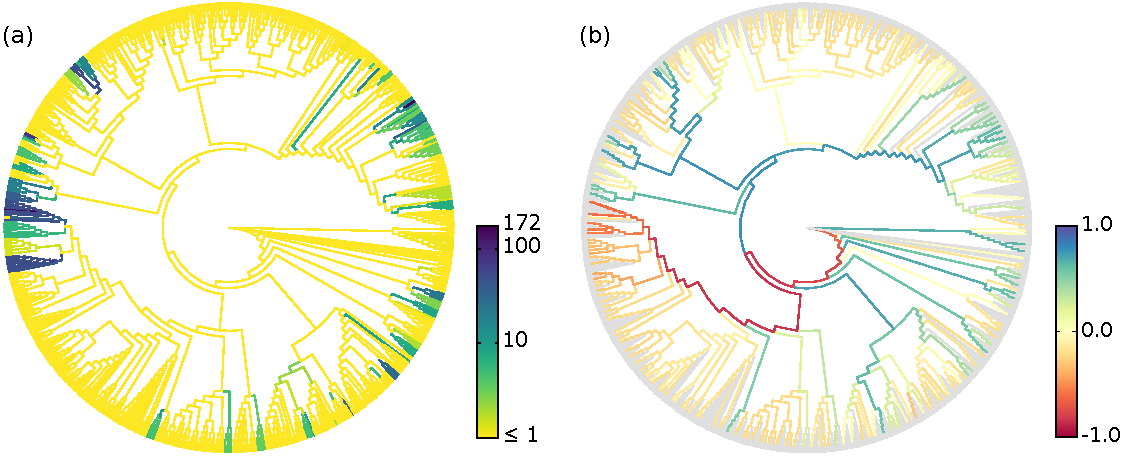
\includegraphics[width=\linewidth]{img/var_cor.pdf}
    \begin{subfigure}{0pt}
        \phantomcaption
        \label{fig:var_cor:sub:em_varl}
    \end{subfigure}
    \begin{subfigure}{0pt}
        \phantomcaption
        \label{fig:var_cor:sub:ei_var}
    \end{subfigure}
    \caption[Examples of Edge Dispersion and Edge Correlation]{
        \textbf{Examples of Edge Dispersion and Edge Correlation.}
        We applied our novel visualization methods to the \ac{BV} dataset
        to compare them to the existing examinations of the data.
%         See \cite{Srinivasan2012} for details of the dataset and its interpretation.
        \subref{fig:var_cor:sub:em_varl}
        Edge Dispersion, measured as the standard deviation of the edge masses across samples, logarithmically scaled.
        \subref{fig:var_cor:sub:ei_var}
        Edge Correlation, in form of Spearman's Rank Correlation Coefficient
        between the edge imbalances and the Nugent score.
        Tip edges are gray, because they do not have a meaningful imbalance.
        This example also shows the characteristics of edge masses and edge imbalances:
        The former highlights individual edges, the latter paths to clades.
%         Note that in this case, both methods highlight similar parts of the tree.
    }
    \label{fig:var_cor}
\end{figure}

% ######################################################################################################################
%         Edge Correlation
% ######################################################################################################################

\section{Edge Correlation}
\label{ch:Visualization:sec:EdgeCorrelation}

In addition to the per-edge masses, the Edge Correlation further
takes a specific meta-data feature into account, that is, a column of the meta-data matrix.
The Edge Correlation is calculated as the correlation between each edge column and the feature column,
for example by using the Pearson Correlation Coefficient or Spearman's Rank Correlation Coefficient \cite{Everitt2010}.
This yields a per-edge correlation of the placement masses or imbalances with the meta-data feature,
and can again be visualized via color coding of the edges.
It is inexpensive to calculate and hence scales well to large datasets.
As typical correlation coefficients are within $[ -1.0, 1.0 ]$, there is again no need for further normalization.
This yields a tree where edges or clades with either a high linear or monotonic correlation
with the selected meta-data feature are highlighted.
\figref{fig:var_cor:sub:ei_var} shows an example of this method.
In contrast to Edge PCA \cite{Matsen2011a} that can use meta-data features to annotate samples in its scatter plots,
our Edge Correlation method directly represents the influence of a feature on the branches or clades of the tree.
It can thus, for example, help to identify and visualize dependencies
between species abundances and environmental factors such as temperature or nutrient levels.
Again, the choice of normalization strategy is important to draw meaningful conclusions.
However, the correlation is \emph{not} calculated between samples or sequence abundances.
% the masses are not put into correlation with each other
Hence, even when using normalized samples, %that is, working with compositional data,
the pitfalls regarding correlations of compositional data \cite{Lovell2015} do not apply here.

% correlation: not correlating masses to each other, so the caveat does not apply.
% not setting compositional values in correlation with each other, so the pitfall schnappt nicht zu
% we simply say: relatively more on that branch, if higher metadata value

% ######################################################################################################################
%         Results
% ######################################################################################################################

\section{Results}
\label{ch:Visualization:sec:Results}

% ----------------------------------------------------------------------------------------------------------------------
%     BV Dataset
% ----------------------------------------------------------------------------------------------------------------------

\subsection{BV Dataset}
\label{ch:Visualization:sec:Results:sub:BVDataset}

We re-analyzed the \ac{BV} dataset by inferring a tree from the original reference sequence set
and conducting phylogenetic placement of the \num{220} samples.
The characteristics of this dataset were already explored in \cite{Srinivasan2012} and \cite{Matsen2011a}.
We use it here to give exemplary interpretations of our Edge Dispersion and Edge Correlation methods,
and to evaluate them in comparison to existing methods.

\figref{fig:var_cor} shows our novel visualizations of the \ac{BV} dataset.
Edge Dispersion is shown in \figref{fig:var_cor:sub:em_varl},
% using the standard deviation of the edge masses, logarithmically scaled.
while \figref{fig:var_cor:sub:ei_var} shows Edge Correlation with the so-called Nugent score. % with the edge imbalances.
The Nugent score \cite{Nugent1991} is a clinical standard for the diagnosis of Bacterial Vaginosis,
ranging from \num{0} (healthy) to \num{10} (severe illness).
The connection between the Nugent score and the abundance of placements on particular edges
was already explored in \cite{Matsen2011a}, but only visualized indirectly (i.e., not on the \ac{RT} itself).
For example, Figure~6 of the original study plots the first two Edge PCA components colorized by the Nugent score.
We recalculated this figure for comparison in \figref{fig:kmeans_all:sub:epca_ns}.
In contrast, our Edge Correlation measure directly reveals the connection between Nugent score and placements on the reference tree:
The clade on the left hand side of the tree, to which the red and orange branches lead to,
are \taxonname{Lactobacillus iners} and \taxonname{Lactobacillus crispatus}, respectively,
which were identified in \cite{Srinivasan2012} to be associated with a healthy vaginal microbiome.
Thus, their presence in a sample is anti-correlated with the Nugent score, which is lower for healthy subjects.
The branches leading to this clade are hence colored in red.
On the other hand, there are several other clades that exhibit a positive correlation with the Nugent score,
that is, were green and blue paths lead to in the figure,
again a finding already reported in \cite{Srinivasan2012}.

Both trees in \figref{fig:var_cor} highlight the same parts of the tree:
The dark branches with high deviation in \figref{fig:var_cor:sub:em_varl} represent clades
attached to either highly correlated (blue) or anti-correlated (red) paths \figref{fig:var_cor:sub:ei_var}.
This indicates that edges that have a high dispersion
also vary between samples of different Nugent score.
% This indicates that both methods reveal the clades that are relevant for discriminating samples of this dataset.

We further compared our methods to the visualization of Edge PCA components on the reference tree.
To this end, we recalculated Figures 4 and 5 of \cite{Matsen2011a},
and visualized them with our color scheme in \figref{fig:epca} for ease of comparison.
They show the first two components of Edge PCA, mapped back to the \ac{RT}.
The first component %, \figref{fig:epca:sub:comp1},
reveals that the \taxonname{Lactobacillus} clade represents the axis with the highest heterogeneity across samples,
while the second component%, \figref{fig:epca:sub:comp2},
further distinguishes between the two aforementioned clades within \taxonname{Lactobacillus}.
Edge Correlation also highlights the \taxonname{Lactobacillus} clade as shown in \figref{fig:var_cor:sub:ei_var},
but does not distinguish further between its sub-clades.
This is because a high Nugent score is associated
with a high abundance of placements in either of the two relevant \taxonname{Lactobacillus} clades.
% In other words, Edge Correlation only reveals information that is associated with the used meta-data feature.

Further examples of variants of Edge Dispersion and Edge Correlation on this dataset
are shown in \figref{fig:all_dispersions} and \figref{fig:all_nugent}.
We also conducted Edge Correlation using Amsel's criteria \cite{Amsel1983} and the vaginal pH value as shown in \figref{fig:amsel_ph},
both of which were used in \cite{Srinivasan2012} as additional indicators of Bacterial Vaginosis.
We again found similar correlations compared to the Nugent score.

% ----------------------------------------------------------------------------------------------------------------------
%     Tara Dataset
% ----------------------------------------------------------------------------------------------------------------------

\subsection{Tara Oceans Dataset}
\label{ch:Visualization:sec:Results:sub:TaraDataset}

We analyzed the \ac{TO} dataset to provide further exemplary use cases for our visualization methods.
To this end, we used the unconstrained \taxonname{Eukaryota} \ac{RT} with \num{2059} taxa
as provided by our Automatic Reference Tree method \cite{Czech2018}.
The meta-data features of this dataset that best lend themselves to our methods are the sensor values for
chlorophyll, nitrate, and oxygen concentration, as well as the salinity and temperature of the water samples.
Other available meta-data features such as longitude and latitude are available,
but would require more involved methods.
This is because geographical coordinates yield pairwise distances between samples,
whose integration into our correlation analysis methods is challenging.
The Edge Correlation of the \num{370} samples with the nitrate concentration, the salinity, the chlorophyll concentration,
and the water temperature are shown in \figref{fig:tara_correlation}.

We selected the diatoms and the animals as two exemplary clades for closer examination of the results.
In particular, the diatoms show a high correlation with the nitrate concentration,
as well as an anti-correlation with salinity, which represent well-known relationships \cite{Lozupone2007,Potapova2011}.
See \figref{fig:tara_correlation} for details.
These findings indicate that the method is able to identify known relationships.
It will therefore also be useful to investigate or discover
insights of novel relationships between sequence abundances and environmental parameters.

% In both cases, the \taxonname{Diatoms} exhibit the most obvious correlation with those meta-data features.
% Diatoms are mainly photosynthetic, and thus rely on nitrogen,
% which explains the high correlating of their clade as shown in \figref{fig:tara_correlation:sub:nitrate}.
% On the other hand, they prefer environments with low salt concentrations,
% which is indicated by the anti-correlation in \figref{fig:tara_correlation:sub:salinity}.

% ----------------------------------------------------------------------------------------------------------------------
%     Performance
% ----------------------------------------------------------------------------------------------------------------------

\subsection{Performance}
\label{ch:Visualization:sec:Results:sub:Performance}

Both methods (Edge Dispersion and Edge Correlation) are computationally inexpensive, and thus applicable to large datasets.
The calculation of the above visualizations took about \SI{30}{\second} each,
which were mainly required for reading in the data.
% In summary, Edge Dispersion is a simple first exploratory tool for visualizing heterogeneity of placements across samples,
% while Edge Correlation is able to directly visualize meta-data features on the \acl{RT}.
Furthermore, in order to scale to large datasets, we reimplemented Edge PCA,
which was originally implemented as a command in the \toolname{guppy} program \cite{Matsen2010}.
For the \ac{BV} dataset with \num{220} samples,
\toolname{guppy} required \SI{9}{\minute} and used \SI{2.2}{\giga\byte} of memory,
while our implementation only required \SI{33}{\second} on a single core, using less than \SI{600}{\mega\byte} of main memory.
For the \ac{HMP} dataset, as it is only single-threaded, \toolname{guppy} took \num{11} days and \SI{75.1}{\giga\byte} memory,
while our implementation needed \SI{7.5}{\minute} on \num{16} cores and used \SI{43.5}{\giga\byte} memory.

% guppy memory timeline
% 10min: 2.0 GB
% 20min: 2.7 GB
% 30min: 3.3 GB
% projection from reading speed: 102.8 GB in a few days

% bv dataset: 440mb. hmp dataset: 20gb
% projection from bv dataset: 100 GB, 8 hours

% speed and mem of our implementation of edge pca vs guppy:
% guppy single core
%     Elapsed (wall clock) time (h:mm:ss or m:ss): 9:01.12
%     Maximum resident set size (kbytes): 2,233,512
% genesis single core
%     Elapsed (wall clock) time (h:mm:ss or m:ss): 0:33.61
%     Maximum resident set size (kbytes): 574,284
% genesis 4 cores
%     Elapsed (wall clock) time (h:mm:ss or m:ss): 0:23.25
%     Maximum resident set size (kbytes): 603,264
%
% single core: 16.1 times faster, 0.26 times memory

% ######################################################################################################################
%         Conclusion and Outlook
% ######################################################################################################################

\section{Conclusion and Outlook}
\label{ch:Visualization:sec:ConclusionOutlook}

Edge Dispersion highlights branches of the phylogenetic tree that exhibit variations in the number of placements,
and thus allows to identify regions of the tree with a high placement heterogeneity.
Edge Correlation additionally takes meta-data features into account,
and identifies branches of the tree that correlate with quantitative features,
such as the temperature or the pH value of the environmental samples.
These methods complement existing methods such as Edge PCA,
and are data exploration tools that can help unravel new patterns in phylogenetic placement data.
The variants of the methods presented here are hence best used in combination with each other.

% ######################################################################################################################
%         Supplement
% ######################################################################################################################

% ======================================================================================================================
%     Edge Dispersion
% ======================================================================================================================

\begin{figure}[!ht]
    \centering
%     \includegraphics[width=\linewidth]{img/all_dispersions.pdf}
    \begin{subfigure}{0pt}
        \phantomcaption
        \label{fig:all_dispersions:sub:em_var}
    \end{subfigure}
    \begin{subfigure}{0pt}
        \phantomcaption
        \label{fig:all_dispersions:sub:em_varc}
    \end{subfigure}
    \begin{subfigure}{0pt}
        \phantomcaption
        \label{fig:all_dispersions:sub:em_iod}
    \end{subfigure}
    \begin{subfigure}{0pt}
        \phantomcaption
        \label{fig:all_dispersions:sub:ei_var}
    \end{subfigure}
    \caption[Examples of variants of Edge Dispersion]{
        \textbf{Examples of variants of Edge Dispersion.}
        We re-analyzed the \ac{BV} dataset to show variants of our Edge Dispersion method.
        All subfigures highlight the same branches and clades as found by other methods such as Edge PCA.
        The method is useful as a first exploratory tool to detect placement heterogeneity across samples.
        In contrast to Edge Correlation, it can however not explain the reasons of heterogeneity.
        % Sub (A)
        Subfigure~\subref{fig:all_dispersions:sub:em_var}
        shows the standard deviation of the absolute edge masses, without any further processing.
        It is striking that one outlier, marked with an arrow, is dominating,
        thus hiding the values on less variable edges.
        This outlier occurs at the species \taxonname{Prevotella bivia} in one of the \num{220} samples,
        where \num{2 781} out of \num{2 782} sequences in the sample have placement mass on that branch.
        Upon close examination, this outlier can also be seen in Figure 1D of \cite{Srinivasan2012},
        but is less apparent there.
        % Sub (B)
        Subfigure~\subref{fig:all_dispersions:sub:em_varc}
        is identical to \figref{fig:var_cor:sub:em_varl} of the main text
        and shows the standard deviation again, but this time using logarithmic scaling,
        thus revealing more details on the edges with lower placement mass variance.
        Furthermore, when comparing it to \figref{fig:all_nugent:sub:srcc_em},
        we see that the same clades that exhibit a high correlation or anti-correlation with meta-data there
        are also highlighted here.
        There are only few medium values, which indicates that there are two classes of edges:
        Those which distinguish patients and those who have almost no placement on them at all.
        % Sub (C)
        Subfigure~\subref{fig:all_dispersions:sub:em_iod}
        shows the Index of Dispersion of the edge masses, that is, the variance normalized by the mean.
        Hence, edges with a higher number of placements are also allowed to have a higher variance.
        We again use a logarithmic scale because of the outlier.
        The figure reveals more details on the edges with lower variance, highlighted in medium green colors.
        % Sub (D)
        Subfigure~\subref{fig:all_dispersions:sub:ei_var}
        shows the standard deviation of edge imbalances.
        Because we used imbalances of unit mass samples, the values are already normalized.
        The path to the \taxonname{Lactobacillus} clade is again clearly visible,
        indicating that the placement mass in this clade has a high variance across samples.
        Note that imbalances can be negative; thus, the Index of Dispersion is not applicable to them.
    }
    \label{fig:all_dispersions}
\end{figure}

% the outlier in \ref{fig:all_dispersions:sub:em_var} is:
% taxon 258b-16, branch id 786, species Prevotella bivia.
%
% command to count the occurence of this per samples:
% cd /home/lucas/Projects/bacardi/03_bv/03_epa/orig_queries_jplace_clean
% grep -n " 786," * | cut -c 1-10 | uniq -c > ../count_258b-16_786.txt
%
% outlier sample is p4z1r15.jplace with 2781 of 2782 pqueries that have a placement on that branch!

% ======================================================================================================================
%     Edge Correlation
% ======================================================================================================================

\begin{figure}[hpbt]
    \centering
%     \includegraphics[width=\linewidth]{img/all_nugent.pdf}
    \begin{subfigure}{0pt}
        \phantomcaption
        \label{fig:all_nugent:sub:pcc_em}
    \end{subfigure}
    \begin{subfigure}{0pt}
        \phantomcaption
        \label{fig:all_nugent:sub:pcc_ei}
    \end{subfigure}
    \begin{subfigure}{0pt}
        \phantomcaption
        \label{fig:all_nugent:sub:srcc_em}
    \end{subfigure}
    \begin{subfigure}{0pt}
        \phantomcaption
        \label{fig:all_nugent:sub:srcc_ei}
    \end{subfigure}
    \caption[Examples of variants of Edge Correlation]{
        \textbf{Examples of variants of Edge Correlation.}
        We again use the \ac{BV} dataset, and show the correlation of edge masses and imbalances with the Nugent score.
        The Nugent score measures the severeness of Bacterial Vaginosis,
        and ranges from \num{0} for healthy subjects to \num{10} for heavily affected patients.
        Subfigures \subref{fig:all_nugent:sub:pcc_em} and \subref{fig:all_nugent:sub:pcc_ei} use the
        Pearson Correlation Coefficient, that is, they show the linear correlation with the meta-data feature,
        while subfigures \subref{fig:all_nugent:sub:srcc_em} and \subref{fig:all_nugent:sub:srcc_ei} use
        Spearman's Rank Correlation Coefficient and thus show monotonic correlations.
        Subfigure~\subref{fig:all_nugent:sub:srcc_ei} is identical to \figref{fig:var_cor:sub:ei_var} of the main text.
        All subfigures show red edges or red paths at the \taxonname{Lactobacillus} clade.
        This indicates that presence of placements in this clade is anti-correlated with the Nugent score,
        which is consistent with the findings of \cite{Srinivasan2012} and \cite{Matsen2011a}.
        In other words, presence of \taxonname{Lactobacillus} correlates with a healthy vaginal microbiome.
        On the other hand, blue and green edges, which indicate positive correlation,
        are indicative of edges that correlate to Bacterial Vaginosis.
        The extent of correlation is larger for Spearman's Coefficient,
        indicating that the correlation is monotonic, but not strictly linear.
    }
    \label{fig:all_nugent}
\end{figure}

% ======================================================================================================================
%     Amsel and pH
% ======================================================================================================================

\begin{figure}[hpbt]
    \centering
%     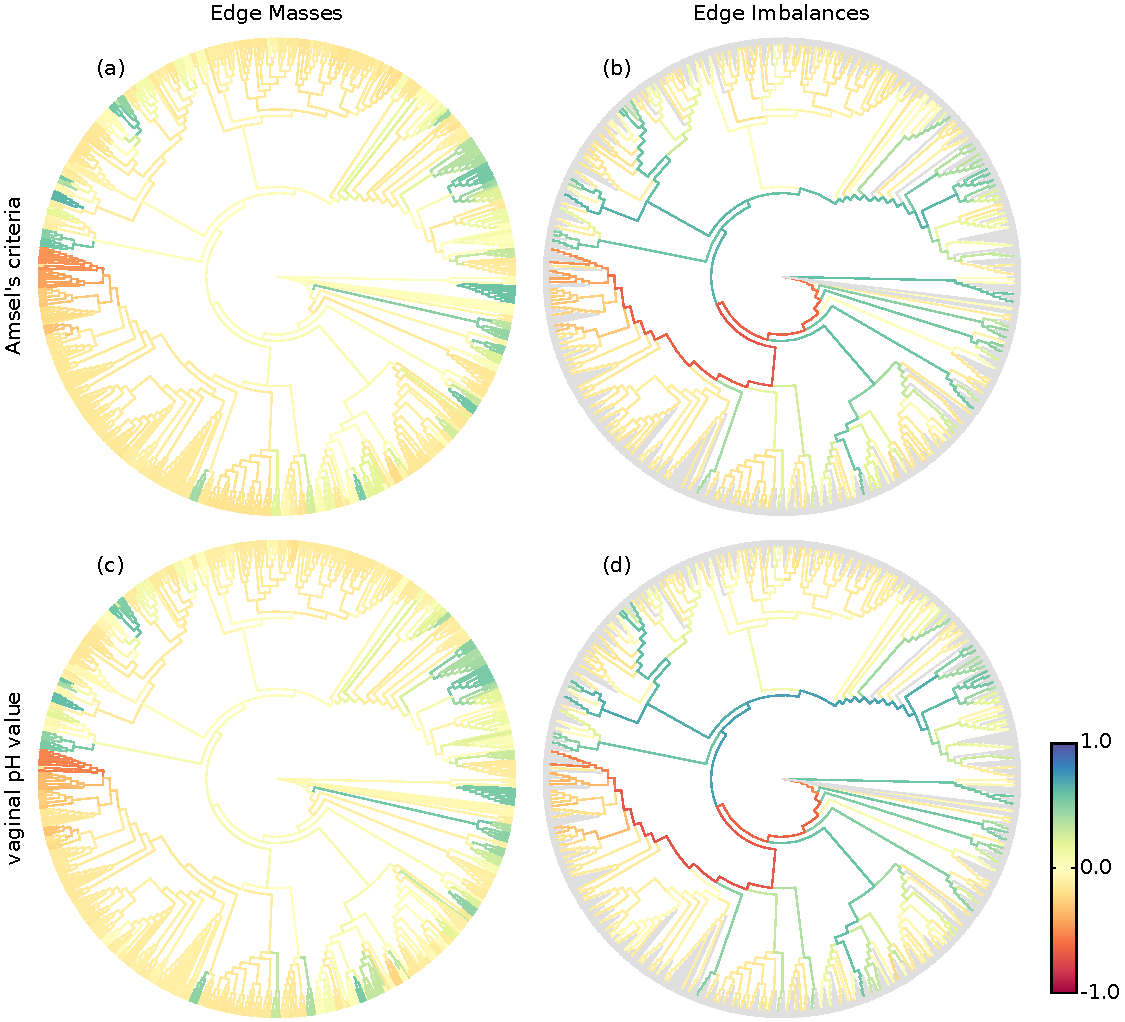
\includegraphics[width=\linewidth]{img/amsel_ph.pdf}
    \begin{subfigure}{0pt}
        \phantomcaption
        \label{fig:amsel_ph:sub:amsel_em}
    \end{subfigure}
    \begin{subfigure}{0pt}
        \phantomcaption
        \label{fig:amsel_ph:sub:amsel_ei}
    \end{subfigure}
    \begin{subfigure}{0pt}
        \phantomcaption
        \label{fig:amsel_ph:sub:ph_em}
    \end{subfigure}
    \begin{subfigure}{0pt}
        \phantomcaption
        \label{fig:amsel_ph:sub:ph_ei}
    \end{subfigure}
    \caption[Edge Correlation with more meta-data features]{
        \textbf{Edge Correlation with more meta-data features.}
        Here, we use additional meta-data features of the \ac{BV} dataset
        to show that Edge Correlation yields consistent results with existing methods.
        In particular, we caltucated Spearman's Coefficient with Amsel's criteria \cite{Amsel1983}
        in subfigures \subref{fig:amsel_ph:sub:amsel_em} and \subref{fig:amsel_ph:sub:amsel_ei},
        as well as with the vaginal pH value
        in subfigures \subref{fig:amsel_ph:sub:ph_em} and \subref{fig:amsel_ph:sub:ph_ei}.
        Both features were also used in \cite{Srinivasan2012} as indicators of Bacterial Vaginosis.
        The figures are almost identical to the ones shown in \figref{fig:all_nugent};
        that is, they yield results that are consistent with the previously used Nugent score,
        as well as consistent with existing methods.
    }
    \label{fig:amsel_ph}
\end{figure}

% ======================================================================================================================
%     Edge PCA
% ======================================================================================================================

\begin{figure}[hpbt]
    \centering
%     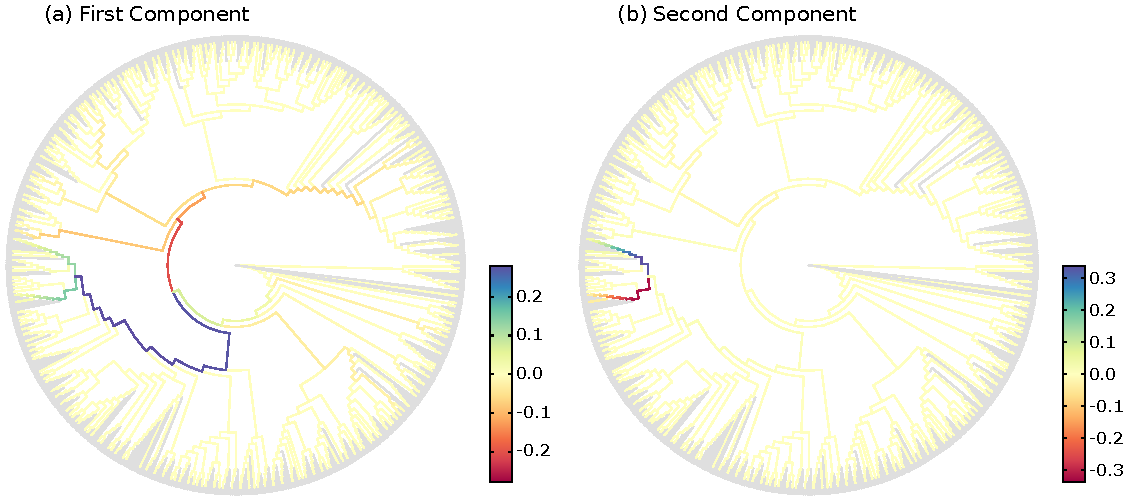
\includegraphics[width=\linewidth]{img/epca.pdf}
    \begin{subfigure}{0pt}
        \phantomcaption
        \label{fig:epca:sub:comp1}
    \end{subfigure}
    \begin{subfigure}{0pt}
        \phantomcaption
        \label{fig:epca:sub:comp2}
    \end{subfigure}
    \caption[Recalculation of the Edge PCA tree visualization]{
        \textbf{Recalculation of the Edge PCA tree visualization.}
        Subfigures~\subref{fig:epca:sub:comp1} and \subref{fig:epca:sub:comp2} are recalculations
        of Figures 4 and 5 of \cite{Matsen2011a}, respectively.
        However, we show them here in our coloring scheme in order to facilitate comparison with other figures.
        The original publication instead uses two colors for a positive and a negative sign of the principal components,
        and branch width to show their magnitude.
        Note that the actual sign is arbitrary, as it is derived from principal components.
        \\
        The figure shows the first two Edge PCA components, visualized on the reference tree.
        This form of visualization is useful to interpret results such as the Edge PCA projection plot
        as shown in \figref{fig:cluster_kmeans:sub:edgepca} of the main text.
        It reveals which edges are mainly responsible for separating the samples into the PCA dimensions.
        Here, the first principal component in \subref{fig:epca:sub:comp1} indicates that the main PCA axis
        separates samples based on the presence of placements in the \taxonname{Lactobacillus} clade,
        which is what the blue and green path leads to.
        The second component in \subref{fig:epca:sub:comp2} then further distinguishes between two species
        in this clade, namely \taxonname{Lactobacillus iners} and \taxonname{Lactobacillus crispatus}.
    }
    \label{fig:epca}
\end{figure}

% ======================================================================================================================
%     Tara Correlation
% ======================================================================================================================

\begin{figure}[hpbt]
    \centering
%     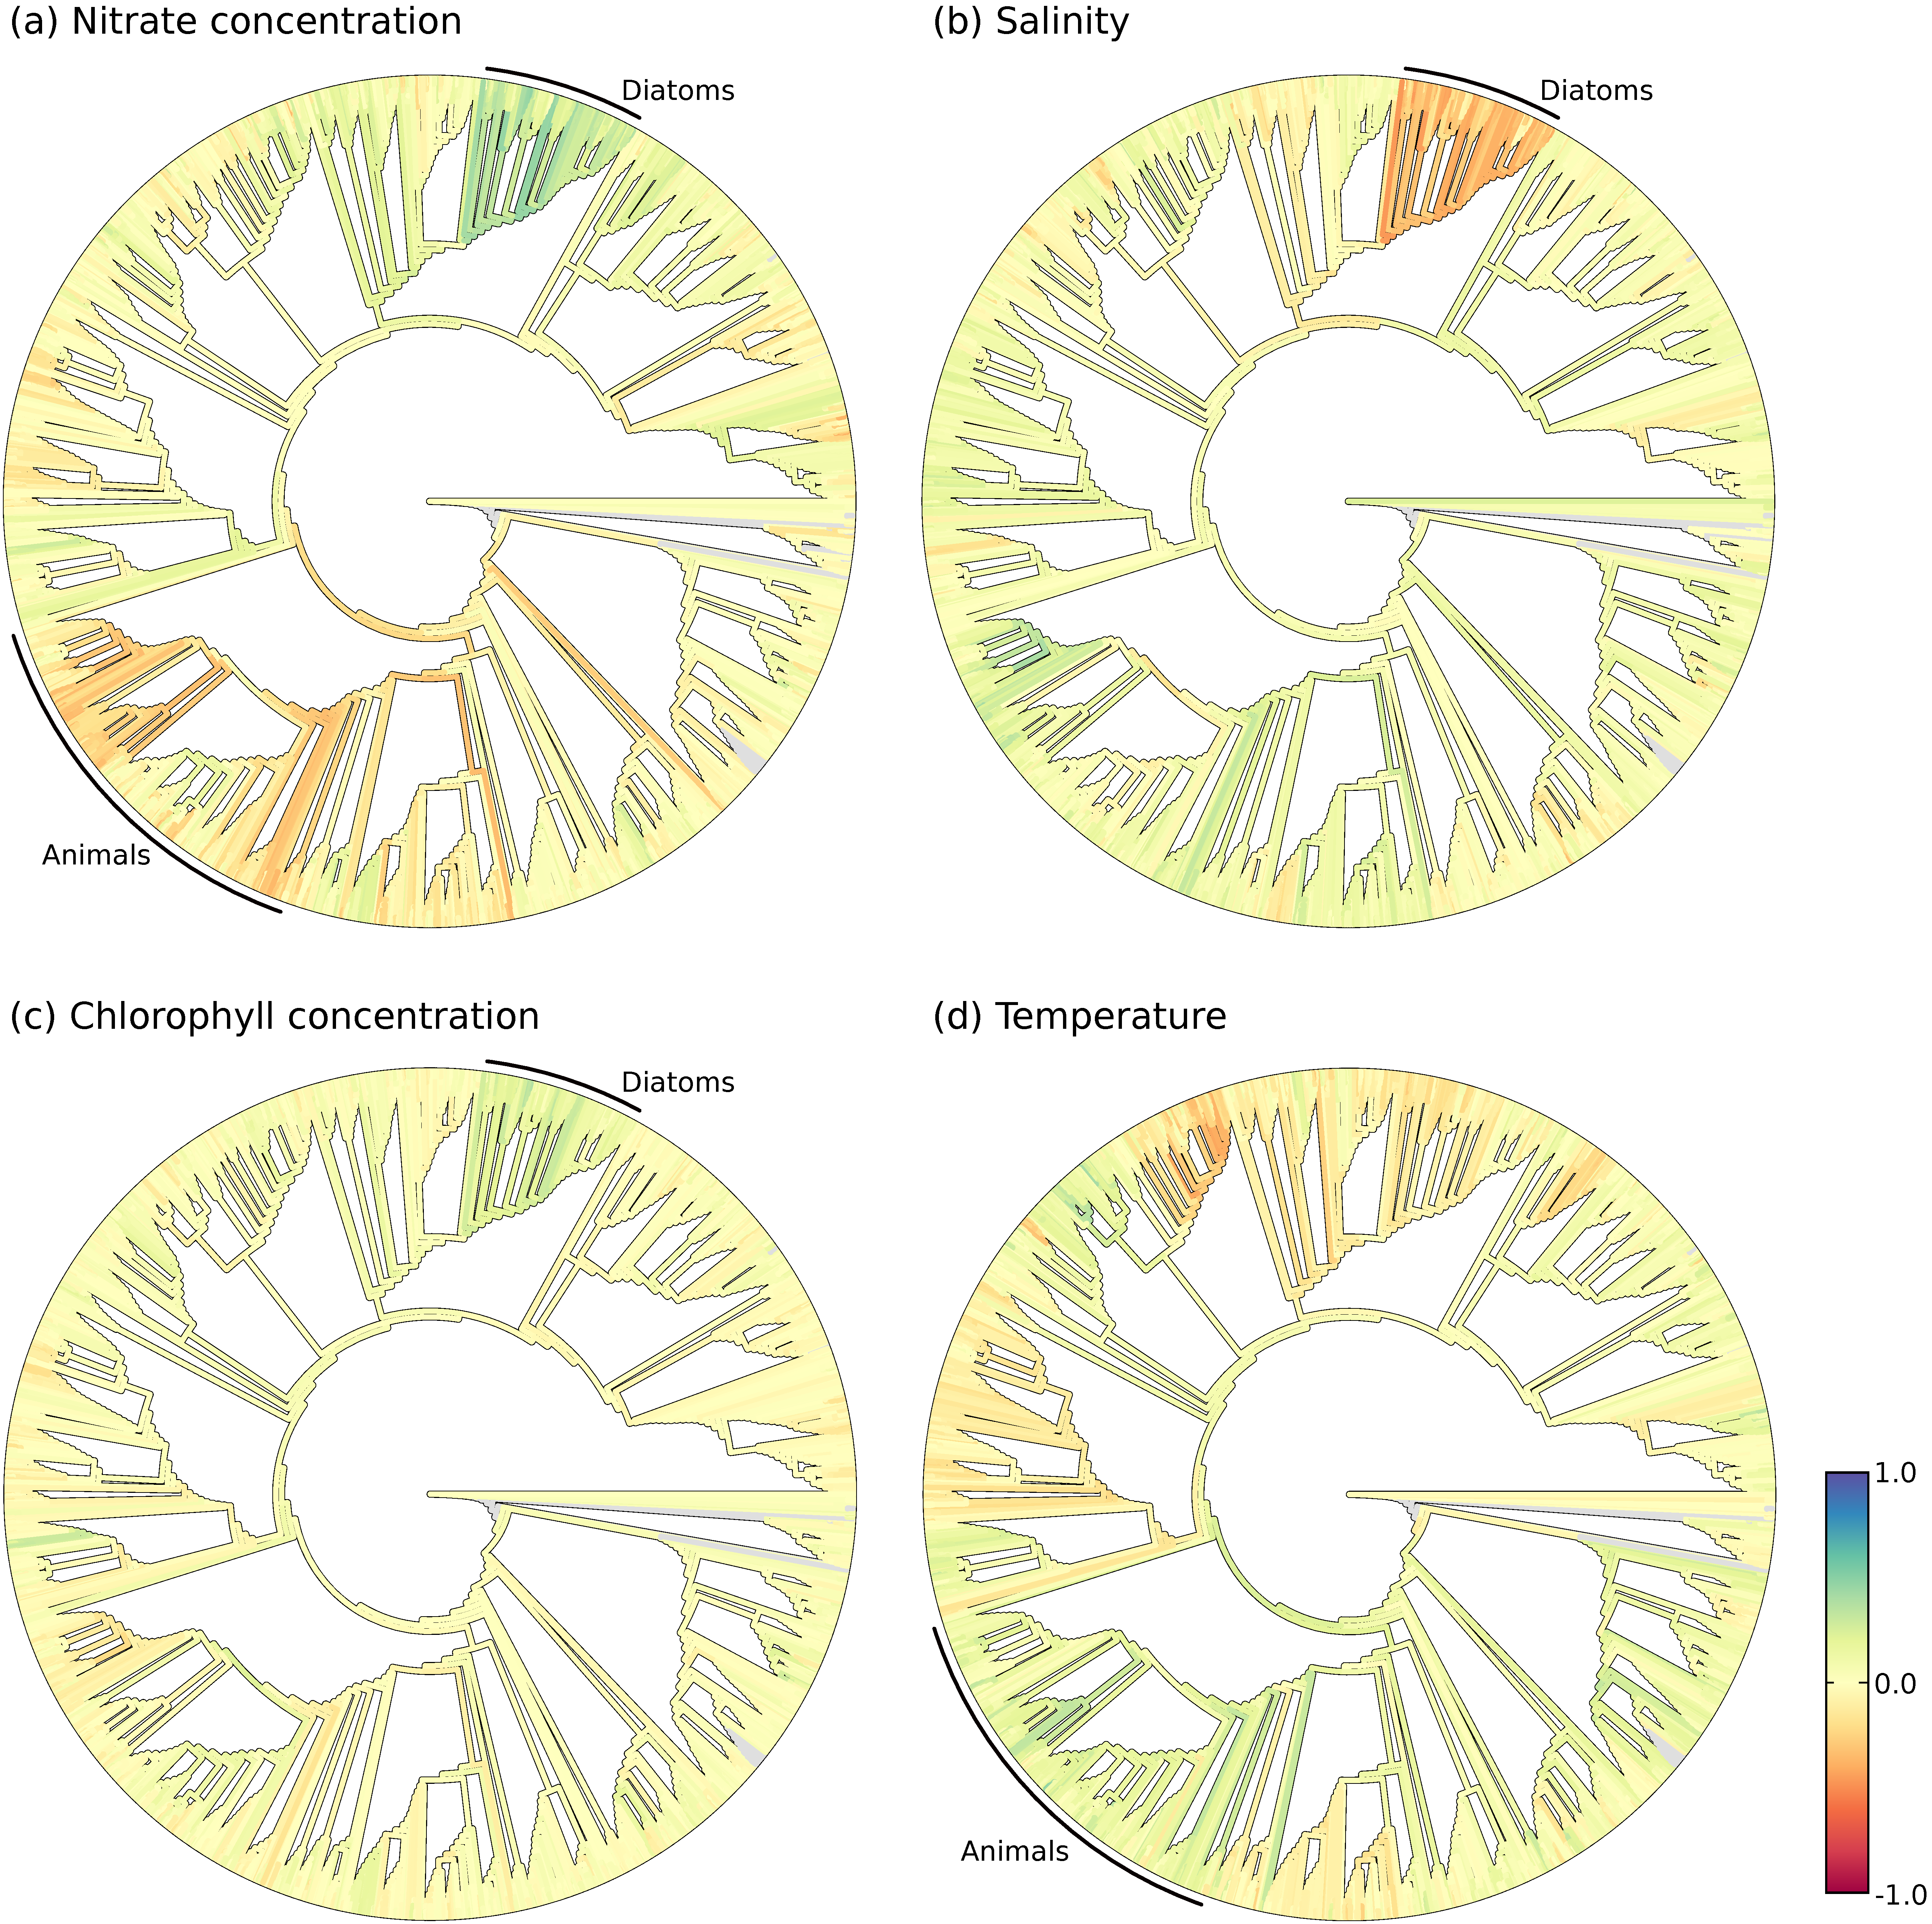
\includegraphics[width=\linewidth]{img/tara_correlation.pdf}
    \begin{subfigure}{0pt}
        \phantomcaption
        \label{fig:tara_correlation:sub:nitrate}
    \end{subfigure}
    \begin{subfigure}{0pt}
        \phantomcaption
        \label{fig:tara_correlation:sub:salinity}
    \end{subfigure}
    \begin{subfigure}{0pt}
        \phantomcaption
        \label{fig:tara_correlation:sub:chlorophyll}
    \end{subfigure}
    \begin{subfigure}{0pt}
        \phantomcaption
        \label{fig:tara_correlation:sub:temperature}
    \end{subfigure}
    \caption[Examples of Edge Correlation using Tara Oceans samples]{
        \textbf{Examples of Edge Correlation using Tara Oceans samples.}
        The figure shows the correlation of Tara Oceans sequence placements with
        \subref{fig:tara_correlation:sub:nitrate} the nitrate,
        \subref{fig:tara_correlation:sub:salinity} the salinity,
        \subref{fig:tara_correlation:sub:chlorophyll} the chlorophyll, and
        \subref{fig:tara_correlation:sub:temperature} the temperature sensor data of each sample.
        The sensor values range from \SI{-2.2}{} to \SI[per-mode=symbol]{33.1}{\micro\mole\per\litre} (nitrate),
        from \SI{33.2}{} to \SI{40.2}{psu} (salt),
        from \SI{-0.02}{} to \SI[per-mode=symbol]{1.55}{\milli\gram\per\cubic\metre} (chlorophyll), and
        from \SI{-0.8}{} to \SI{30.5}{\celsius} (temperature), respectively.
        The negative nitrate and chlorophyll concentrations are
        values below the detection limit of the measurement method (pers.~comm.~with L.~Guidi),
        and hence simply denote low concentrations.
        We used Spearman's Rank Correlation Coefficient,
        and examine two exemplary clades, namely the \taxonname{Animals} and the \taxonname{Diatoms}.
        \\
        Diatoms are mainly photosynthetic, and thus depend on nitrates as key nutrients,
        which is clearly visible by the high correlation of the clade in \subref{fig:tara_correlation:sub:nitrate}.
        Furthermore, the diatoms exhibit positive correlation
        with the chlorophyll concentration \subref{fig:tara_correlation:sub:chlorophyll},
        which again is indicative of their photosynthetic behavior.
        On the other hand, they show a high anti-correlation
        with the salt content \subref{fig:tara_correlation:sub:salinity}.
        Salinity is a strong environmental factor which heavily affects community structures
        and species abundances \cite{Lozupone2007}, particularly diatoms \cite{Potapova2011}.
        \\
        The correlations of the animal clade are less pronounced.
        They exhibit a negative correlation with nitrate \subref{fig:tara_correlation:sub:nitrate},
        as well as an increase in absolute abundance with higher temperatures \subref{fig:tara_correlation:sub:temperature}.
        While these findings are not surprising,
        they show that the method is able to find meaningful relationships in the data.
    }
    \label{fig:tara_correlation}
\end{figure}
